\section{Auswertung}
\label{sec:Auswertung}

\subsection{Bestimmung der Winkelrichtgröße}

Die Messung wird mit einem senkrechten Abstand von ${r=\SI{4.0}{\centi\meter}}$ durchgeführt. 
Der Auslenkwinkel $\varphi$ und die aufgewendete Kraft $F$ sind in \ref{tab:richtgrD} dargestellt, ebenso wie die sich daraus 
ergebenden Werte für die Winkelrichtgröße $D$. 
Sie berechnet sich, wie aus der Theorie zu entnehmen ist, über 
\begin{equation}
    D=\frac{Fr}{\varphi}\:.
\end{equation}

\begin{table}
    \centering
    \caption{Messwerte zur Bestimmung der Winkelrichtgröße.}
    \label{tab:richtgrD}
    \begin{tabular}{c S[table-format=1.2] S[table-format=1.2] S[table-format=2.1]}
        \toprule
        {$\varphi$} & {$\varphi\:/\:\symup{\pi}$} & {$F\:/\:\si{\newton}$} & {$D\:/\:\SI{e-3}{\newton\meter}$} \\
        \midrule
        \ang{26;;}  & 0.14  & 0.19 & 17.3 \\
        \ang{30;;}  & 0.17  & 0.21 & 15.7 \\
        \ang{37;;}  & 0.21  & 0.29 & 17.6 \\
        \ang{45;;}  & 0.25  & 0.41 & 20.9 \\
        \ang{60;;}  & 0.33  & 0.49 & 18.9 \\
        \ang{70;;}  & 0.39  & 0.61 & 19.9 \\
        \ang{81;;}  & 0.45  & 0.70 & 19.8 \\
        \ang{93;;}  & 0.52  & 0.74 & 18.1 \\
        \ang{100;;} & 0.56  & 0.91 & 20.7 \\
        \ang{110;;} & 0.61  & 0.97 & 20.2 \\
        \bottomrule
    \end{tabular}
\end{table}

Somit ergibt sich als experimenteller Wert ${D=\SI{18.9(5)e-3}{\newton\meter}}$ für die Winkelrichtgröße. 
Der Fehler des Mittelwerts berechnet sich über 
\begin{equation}
    \increment D = \sqrt{\frac{1}{N(N-1)}\sum_{i=1}^N (D_i-\bar{D})}
\end{equation}
mit dem arithmetischen Mittel $\bar{D}$. 

\FloatBarrier
\subsection{Bestimmung des Eigenträgheitsmoments der Drillachse}

Im Folgenden sei die Annahme eines nahezu masselosen Stabs, an dem zwei Punktmassen -- demnach ohne Ausdehnung -- 
gleicher Masse ${m=\SI{222.89}{\gram}}$ 
befestigt sind. 
In \ref{tab:I_D} sind die Messwerte entsprechend dargestellt. 
Es besteht ein linearer Zusammenhang zwischen den Quadraten der Periode $T$ und dem Abstand $a$ der Massen:

\begin{equation}
    T^2=\frac{4\symup{\pi}^2}{D}\bigl(I_\text{D} + m(a_1^2+a_2^2)\bigr)=:\frac{4\symup{\pi}^2}{D}(I_\text{D}+ma^2)    
    \label{eqn:Thoch2}
\end{equation} 

\begin{table}
    \centering
    \caption{Messwerte zur Bestimmung des Eigenträgheitsmoments $I_\text{D}$.}
    \label{tab:I_D}
    \begin{tabular}{S[table-format=2.1] S[table-format=2.1] S[table-format=4.1] S[table-format=1.2] S[table-format=2.2]}
        \toprule
        {$a_1\:/\:\si{\centi\meter}$} & {$a_2\:/\:\si{\centi\meter}$} & {$(a_1^2+a_2^2)\:/\:\si{\centi\meter\squared}$} & {$T\:/\:\si{\second}$} & {$T^2\:/\:\si{\second\squared}$} \\
        \midrule
        4.5  & 5.5  &   50.5 & 2.50 & 6.25  \\
        6.5  & 7.5  &   98.5 & 2.93 & 8.58  \\
        8.5  & 9.5  &  162.5 & 3.21 & 10.30 \\
        10.5 & 11.5 &  242.5 & 3.83 & 14.67 \\
        12.5 & 13.5 &  338.5 & 4.16 & 17.31 \\
        14.5 & 15.5 &  450.5 & 4.70 & 22.09 \\
        16.5 & 17.5 &  578.5 & 5.27 & 27.77 \\
        18.5 & 19.5 &  722.5 & 5.79 & 33.52 \\
        20.5 & 21.5 &  882.5 & 6.27 & 39.31 \\
        22.5 & 23.5 & 1058.5 & 6.78 & 45.97 \\
        \bottomrule
    \end{tabular}
\end{table}

Nun werden diese Werte in einem Diagramm aufgetragen. 
Mithilfe linearer Regression lässt sich aus dem Y-Achsenabschnitt $b$ der Eigenträgheitsmoment $I_D$ bestimmen. 
Die Steigung $c$ ergibt sich unter Vergleich mit \eqref{eqn:Thoch2} aus

\begin{gather}
y=b+cx \\
T^2 = \frac{4\symup{\pi}^2}{D}(I_\text{D}+ma^2) \\
\Rightarrow y = T^2, 
\quad b =  \frac{4\symup{\pi}^2}{D} I_\text{D}, 
\quad c = \frac{4\symup{\pi}^2}{D}m ,
\quad x = a^2 
\end{gather}

Unter Zuhilfenahme von \textit{Python 3.7.3} wird die lineare Regression durchgeführt, wie in Abbildung \ref{fig:Thoch2} zu sehen ist, und es ergibt sich der y-Achsenabschnitt~${b=\SI{4.42(25)}{\second\squared}}$
und eine Steigung von ${c=\SI{396.0\pm4.4}{\kilo\gram\per\joule}}$. 
Daraus lässt sich das Eigenträgheitsmoment zu 
\begin{equation}
    I_\text{D}=\frac{D}{4\symup{\pi}^2}b=\frac{m}{c}b=\SI{2.49(14)e-3}{\kilo\gram\meter\squared}
\end{equation}
bestimmen.

\begin{figure}
    \centering
    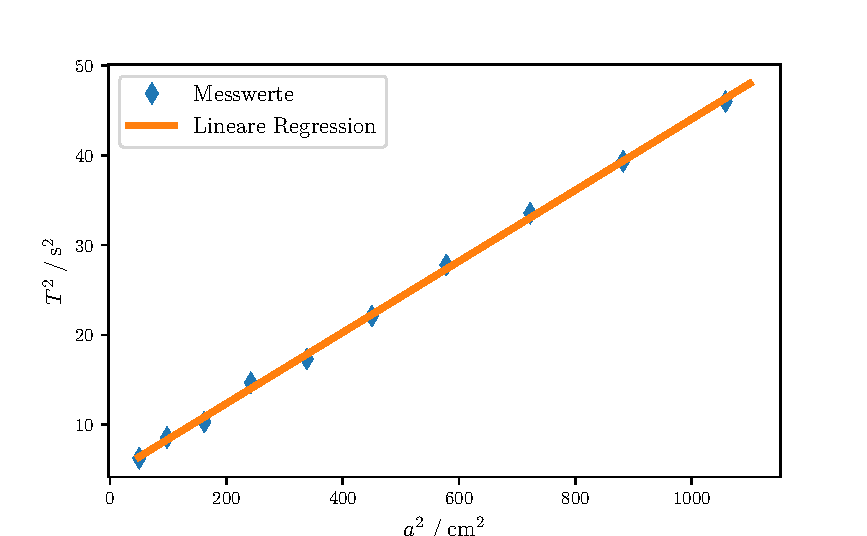
\includegraphics[width=0.8\textwidth]{plots/plot_I_D.pdf}
    \caption{Lineare Regression zur Bestimmung des Eigenträgheitsmoments.}
    \label{fig:Thoch2}
\end{figure}

\FloatBarrier
\subsection{nächste section}

\begin{table}
    \centering
    \caption{Messwerte aller Schwingungsdauern.}
    \label{tab:messSchwing}
    \begin{tabular}{c c c c}
        \toprule
        {T$_{zyl, gross}\:/\:\si{\second}$} & {T$_{zyl, klein}\:/\:\si{\second}$} & {T$_{pose1}\:/\:\si{\second}$} & {T$_{pose2}\:/\:\si{\second}$} \\
        \midrule
        1.08 & 2.31 & 0.38 & 0.92 \\
        1.27 & 2.23 & 0.41 & 0.89 \\
        1.13 & 2.17 & 0.43 & 0.94 \\
        1.18 & 2.30 & 0.39 & 0.91 \\
        1.16 & 2.26 & 0.41 & 0.91 \\
        \bottomrule
    \end{tabular}
\end{table}

\begin{table}
    \centering
    \caption{Messwerte zur Bestimmung der Eigenträgheit.}
    \label{tab:messEigen}
    \begin{tabular}{c c c}
        \toprule
        {T$_{eigen}\:/\:\si{\second}$} & {a$_{m1}\:/\:\si{\centi\meter}$} & {a$_{m2}\:/\:\si{\centi\meter}$} \\
        \midrule
        2.50 & 4.5  & 5.5  \\
        2.93 & 6.5  & 7.5  \\
        3.21 & 8.5  & 9.5  \\
        3.83 & 10.5 & 11.5 \\
        4.16 & 12.5 & 13.5 \\
        4.70 & 14.5 & 15.5 \\
        5.27 & 16.5 & 17.5 \\
        5.79 & 18.5 & 19.5 \\
        6.27 & 20.5 & 21.5 \\
        6.78 & 22.5 & 23.5 \\
        \bottomrule
    \end{tabular}
\end{table}

\begin{table}
    \centering
    \caption{Messunsicherheiten aller Schwingungsdauern.}
    \label{tab:mittelSchwing}
    \begin{tabular}{l c}
        \toprule
        & {T$\:/\:\si{\second}$} \\     % werden Messgrößen kursiv geschrieben? (hier das T)
        \midrule
        Zylinder$_{gross}$  & 2.25$\pm$0.05 \\
        Zylinder$_{klein}$  & 1.16$\pm$0.06 \\
        Holzfigur Pose 1    & 0.40$\pm$0.02 \\
        Holzfigur Pose 2    & 0.91$\pm$0.02 \\
        \bottomrule
    \end{tabular}
\end{table}